\section{ Хеш-функции. Коллизии. Хеш-таблицы.  Хеширование. Фильтр Блюма.}

\begin{definition}
	\textbf{Фильтр Блума} --- вероятностная структура данных позволяющая проверять принадлежность элемента к множеству. 
	При этом существует возможность получить \textbf{ложноположительное} срабатывание (элемента в множестве нет, но структура данных сообщает, что он есть), но не \textbf{ложноотрицательное}.
\end{definition}

То есть данный фильтр даёт два ответа на вопрос о принадлежности элемента к множеству:
\begin{enumerate}
	\item элемент точно не принадлежит множеству,
	\item элемент возможно принадлежит множеству.
\end{enumerate}

Фильтр Блума представляет собой битовый массив из $m$
бит и $k$ различных хеш-функций $h_1 ... h_k$, равновероятно отображающих элементы исходного множества во множество $\{0,1, m-1\}$, соответствующее номерам битов в массиве. 
Изначально, когда структура данных хранит пустое множество, все $m$ бит обнулены.

\begin{figure}[h!]
	\centering
	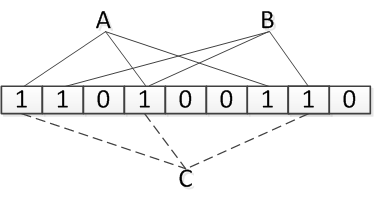
\includegraphics[width=0.4\linewidth]{img_easy/11_1.png}
	\captionsetup{labelformat=empty}
	\caption{Пример фильтра Блума}
\end{figure}

Для добавления элемента $e$ необходимо записать единицы на каждую из позиций $h_1(e)...h_k(e)$ битового массива.

При поиске элемента необходимо проверить наличие единиц на позициях $h_1(e)...h_k(e)$ --- если хотя бы на одной позиции не будет единицы, элемент точно не присутствует в множестве; п